\section{Einleitung}

\begin{equation}
	M = m \frac{V_m}{V}\frac{p_0}{p}\frac{T}{T_0} \label{eq:dampfMolMasse}
\end{equation}

\section{Versuchsteil}
\subsection{Messung der molaren Masse anhand von Dampfdichte}
Im ersten Versuchsteil wird die molare Masse von Ethanol und Cyclohexan bestimmt. Dazu wird genutzt, dass das molare Volumen von idealen Gasen eine konstante ist und sowohl Ethanol als auch Cyclohexan nur geringfügig von diesem Wert abweichen. \\
Es werden geringe Probenmengen von etwa \SI{.1}{\milli\liter} bei Ethanol und \SI{.2}{\milli\liter} bei Cyclohexan mit einer Spritze in einen Glaskolben injiziert. Durch wiegen der Spritze vorm Injizieren und danach wird die Masse des injizierten Stoffes bestimmt. Die Temperatur des Kolbens wird durch ein kochendes Wasserbad konstant auf etwa \SI{100}{\degreeCelsius} gehalten. Da die Siedepunkte von Ethanol und Cyclohexan, wie Tabelle \ref{tab:propEthanolCyclo} entnommen werden kann, deutlich darunter liegen, gehen diese im Kolben in die gasförmige Phase über. Das so verdrängte Volumen kann abgelesen werden und zusammen mit der Probenmasse die Molmasse bestimmt werden. Durch fünf Messungen pro Stoff wird die Unsicherheit verringert.
\begin{figure}[H]
\centering
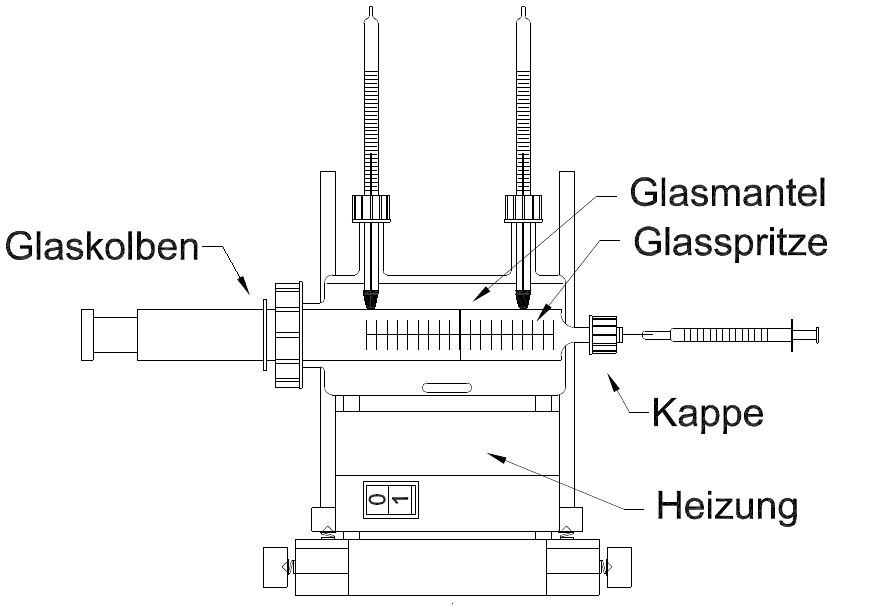
\includegraphics[width=.7\textwidth]{Bilder/aufbau_dampf.png}
\caption[Aufbau]{Versuchsapperatur (Quelle: \cite{anleitung2015})}
\label{fig:aufbau_dampf}
\end{figure}
\subsubsection{Auswertung}

Mit \eqref{eq:dampfMolMasse} lässt sich aus den erfassten Messwerten die molare Masse bestimmen. 

\begin{table}[H]
\centering
\begin{tabular} {c|c|c}
	 & Siedepunkt & Molare Masse \\\hline
	Ethanol & \SI{78,32}{\degreeCelsius} & \SI{46,07}{\g\per\mol} \\
	Cyclohexan & \SI{81}{\degreeCelsius} & \SI{84,16}{ \g\per\mol}
\end{tabular}
\caption{Stoffeigenschaften von Ethanol und Cyclohexan (Quellen: \cite{wiki:ethanol,wiki:cyclohexan})}
\label{tab:propEthanolCyclo}
\end{table} 


\section{Diskussion} % !!!!